As a next topic to uncover goes the one related to the database structure.
Proper database structure is to be of very high priority, since it influences on the project as a whole,
starting from performance point of view and many other aspects.
When we say performance, we mean such a design of database that there is an opportunity to include required indexes,
depending on regularity of any particular request.
So, as the main topic of current thesis is implementation of Instant messaging system, we can list the following
general entities to be added to database schema.

\begin{itemize}
    \item \textbf{Users.} Table stores information about user.
    Table contains following columns:
    \begin{itemize}
        \item Id VARCHAR(36) -- Id of the user, primary key, GUID\@.
        \item UserName VARCHAR(50) -- Unique Username.
        \item NormalizedUserName VARCHAR(50) -- Unique Username in upper case.
        \item DisplayName VARCHAR(50) -- Name of the user, displayed to others.
        \item Bio VARCHAR(250) -- User's short biography, visible to others.
        \item Image VARCHAR(36) -- User's profile picture, visible to others.
        \item Email VARCHAR(120) -- User's email address, not public.
        \item EmailConfirmed BOOLEAN -- Flag that indicates if user has confirmed his email address.
        \item PhoneNumber VARCHAR(50) -- User's phone number.
        \item PhoneNumberConfirmed BOOLEAN -- Flag that indicates if user has confirmed his phone number.
        \item PhoneVerificationCode INTEGER -- Code sent to user in order to confirm phone number.
        \item PasswordHash VARCHAR(60) -- Hashed password.
        \item CreatedAt DATETIME -- Indicates the date and time user has been registered.
        \item UpdatedAt DATETIME -- Indicates the date and time user has updated his record.
    \end{itemize}
    \item \textbf{User Personal Information.} Table stores additional but not required info about user.
    Relation one-to-one with Users, foreign key is UserId, GUID\@.
    Table contains following columns:
    \begin{itemize}
        \item UserId VARCHAR(36) -- Foreign key to the Users table, GUID\@.
        \item FirstName VARCHAR(120) -- First name of user.
        \item LastName VARCHAR(120) -- Last name of user.
        \item BirthDay DATETIME -- Birth day of user.
        \item WebSite VARCHAR(120) -- Web site of user.
        \item Address VARCHAR(120) -- Residence address of user.
        \item Facebook VARCHAR(120) -- Facebook nickname of user.
        \item Twitter VARCHAR(120) -- Twitter nickname of user.
        \item Instagram VARCHAR(120) -- Instagram nickname of user.
        \item LinkedIn VARCHAR(120) -- LinkedIn nickname of user.
        \item ProfilePicture VARCHAR(36) -- Avatar of user.
    \end{itemize}
    \item \textbf{UserContacts.} Table stores the contacts of current user.
    Relation between tables Users and UserContacts is one-to-many, foreign key UserId.
    Table contains following columns:
    \begin{itemize}
        \item ContactId VARCHAR(36) -- Id of current user's contact, GUID\@.
        \item UserId VARCHAR(36) -- Id of current user, GUID\@.
    \end{itemize}
    \item \textbf{Chats.} In order to communicate with other people it is essentially to have a chat room.
    Our implementation provides chat rooms of the four types.
    Direct chat -- chat room between only two members.
    Public channel -- chat room for multiple members, each member can send and read messages.\ It displayed in search results.
    Readonly channel -- channel for multiple members, however only the owner can send messages.\ It displayed in search results.
    Private channel -- channel for multiple members, can be joined only by invite link.
    Each user can have a numerous various chats, however, each chat has a multiple members, at least 2 as the case of direct chat.
    Therefore, we consider a many-to-many relation between user and chats via intermediate table UserChats.
    We discuss UserChats relation in foregoing part.
    Continuing with Chats table, it contains the following columns:
    \begin{itemize}
        \item Id VARCHAR(36) -- Id of the chat, primary key, GUID.
        \item ChatInfoId VARCHAR(36) -- Since we have a four types of channels, which has a common subset of data,
        the different data is moved to another table, so it could be joined depending on chat type.
        For instance, any chat type except direct one would require to join additional data in order to display the chat properly.
        \item Title VARCHAR(50) -- Simply, the title of the chat.
        \item Image VARCHAR(36) -- Picture of the chat.\ Displayed in search results etc.
        \item ChatType ENUM -- The type of the chat, e.g direct chat, public channel, readonly channel, private channel.
        \item CreatedAt DATETIME -- Indicates the date and time chat has been created.
        \item UpdatedAt DATETIME -- Indicates the date and time chat has been updated.
    \end{itemize}
    \item \textbf{UserChats.} Table that considered as composite key of the many-to-many relation between Users and Chats tables.
    Over that, contains an enum value that indicates user's role in the chat.
    We assume the following user roles in the system:
    \begin{itemize}
        \item Owner -- the creator of the chat.
        Has an ultimate privileges.
        \item Administrator -- designated by the owner user, which has adjustable privileges.
        \item Moderator -- designated by administrator user, which has adjustable privileges.
        \item User -- default role assigned to the user on join the chat.
    \end{itemize}
    Despite that, the UserChats table contains the following columns:
    \begin{itemize}
        \item ChatId VARCHAR(36) -- Foreign key to the Chats table, GUID\@.
        \item UserId VARCHAR(36) -- Foreign key to the Users table, GUID\@.
        \item RoleId ENUM -- Indicates the user role in the chat, e.g Owner, Administrator, Moderator, User.
    \end{itemize}
    \item \textbf{Chat Info.} Table contains additional data related to the chat.
    This table is created since that we have four types of chats, namely, direct chat, public channel,
    readonly channel, private channel.
    These four types has a common data between each other.
    Common data between chat types is Chats table itself.
    One would advise to store the chats in a single table per chat type, however it is very costly approach, since there
    would be at least four joins per request.
    Note that every chat type except direct chat requires an additional data to be displayed, that is Chat Info.
    Contains following columns:
    \begin{itemize}
        \item Id VARCHAR(36) -- Id of the chat information, primary key, GUID\@.
        \item Description VARCHAR(120) -- Description of the chat.
        \item Tag VARCHAR(20) -- Unique identifier of the chat.
        \item MembersCount INTEGER -- Count of members in the chat.
    \end{itemize}
    \item \textbf{Messages.} Table that keeps messages and related data.
    Each chat has a multiple messages, however one message must belong only to single and defined chat,
    therefore relation between Chats and Messages is one-to-many, foreign key ChatId.
    From other side, each User has a multiple messages, however single message should belong to single author,
    therefore, we consider one-to-mane relation between Users and Messages, foreign key UserId.
    Messages table contains following columns:
    \begin{itemize}
        \item Id VARCHAR(36) -- Id of the message, primary key, GUID\@.
        \item ChatId VARCHAR(36) -- Foreign key to the Chats table, GUID\@.
        \item UserId VARCHAR(36) -- Foreign key to the Users table, GUID\@.
        \item Content VARCHAR(300) -- Content of the message.
        \item IsRead BOOLEAN -- Indicates whenever message has been read by another user.
        \item CreateAt DATETIME -- Time when the message has been created.
        \item UpdatedAt DATETIME -- Time when the message has been updated.
    \end{itemize}
    \item \textbf{Refresh Tokens.} Table stores refresh tokens.
    \begin{itemize}
        \item Id VARCHAR(36) -- Id of the token, primary key, GUID\@.
        \item UserId VARCHAR(39) -- Foreign key to the Users table, GUID\@.
        \item RefreshToken VARCHAR(60) -- Refresh token itself.
        \item Expires DATETIME -- Expiration date of refresh token.
        \item CreatedAt DATETIME -- Date when token has been created.
    \end{itemize}
\end{itemize}
Following diagram demonstrates the database structure.
\begin{figure}[H]
    \centering
    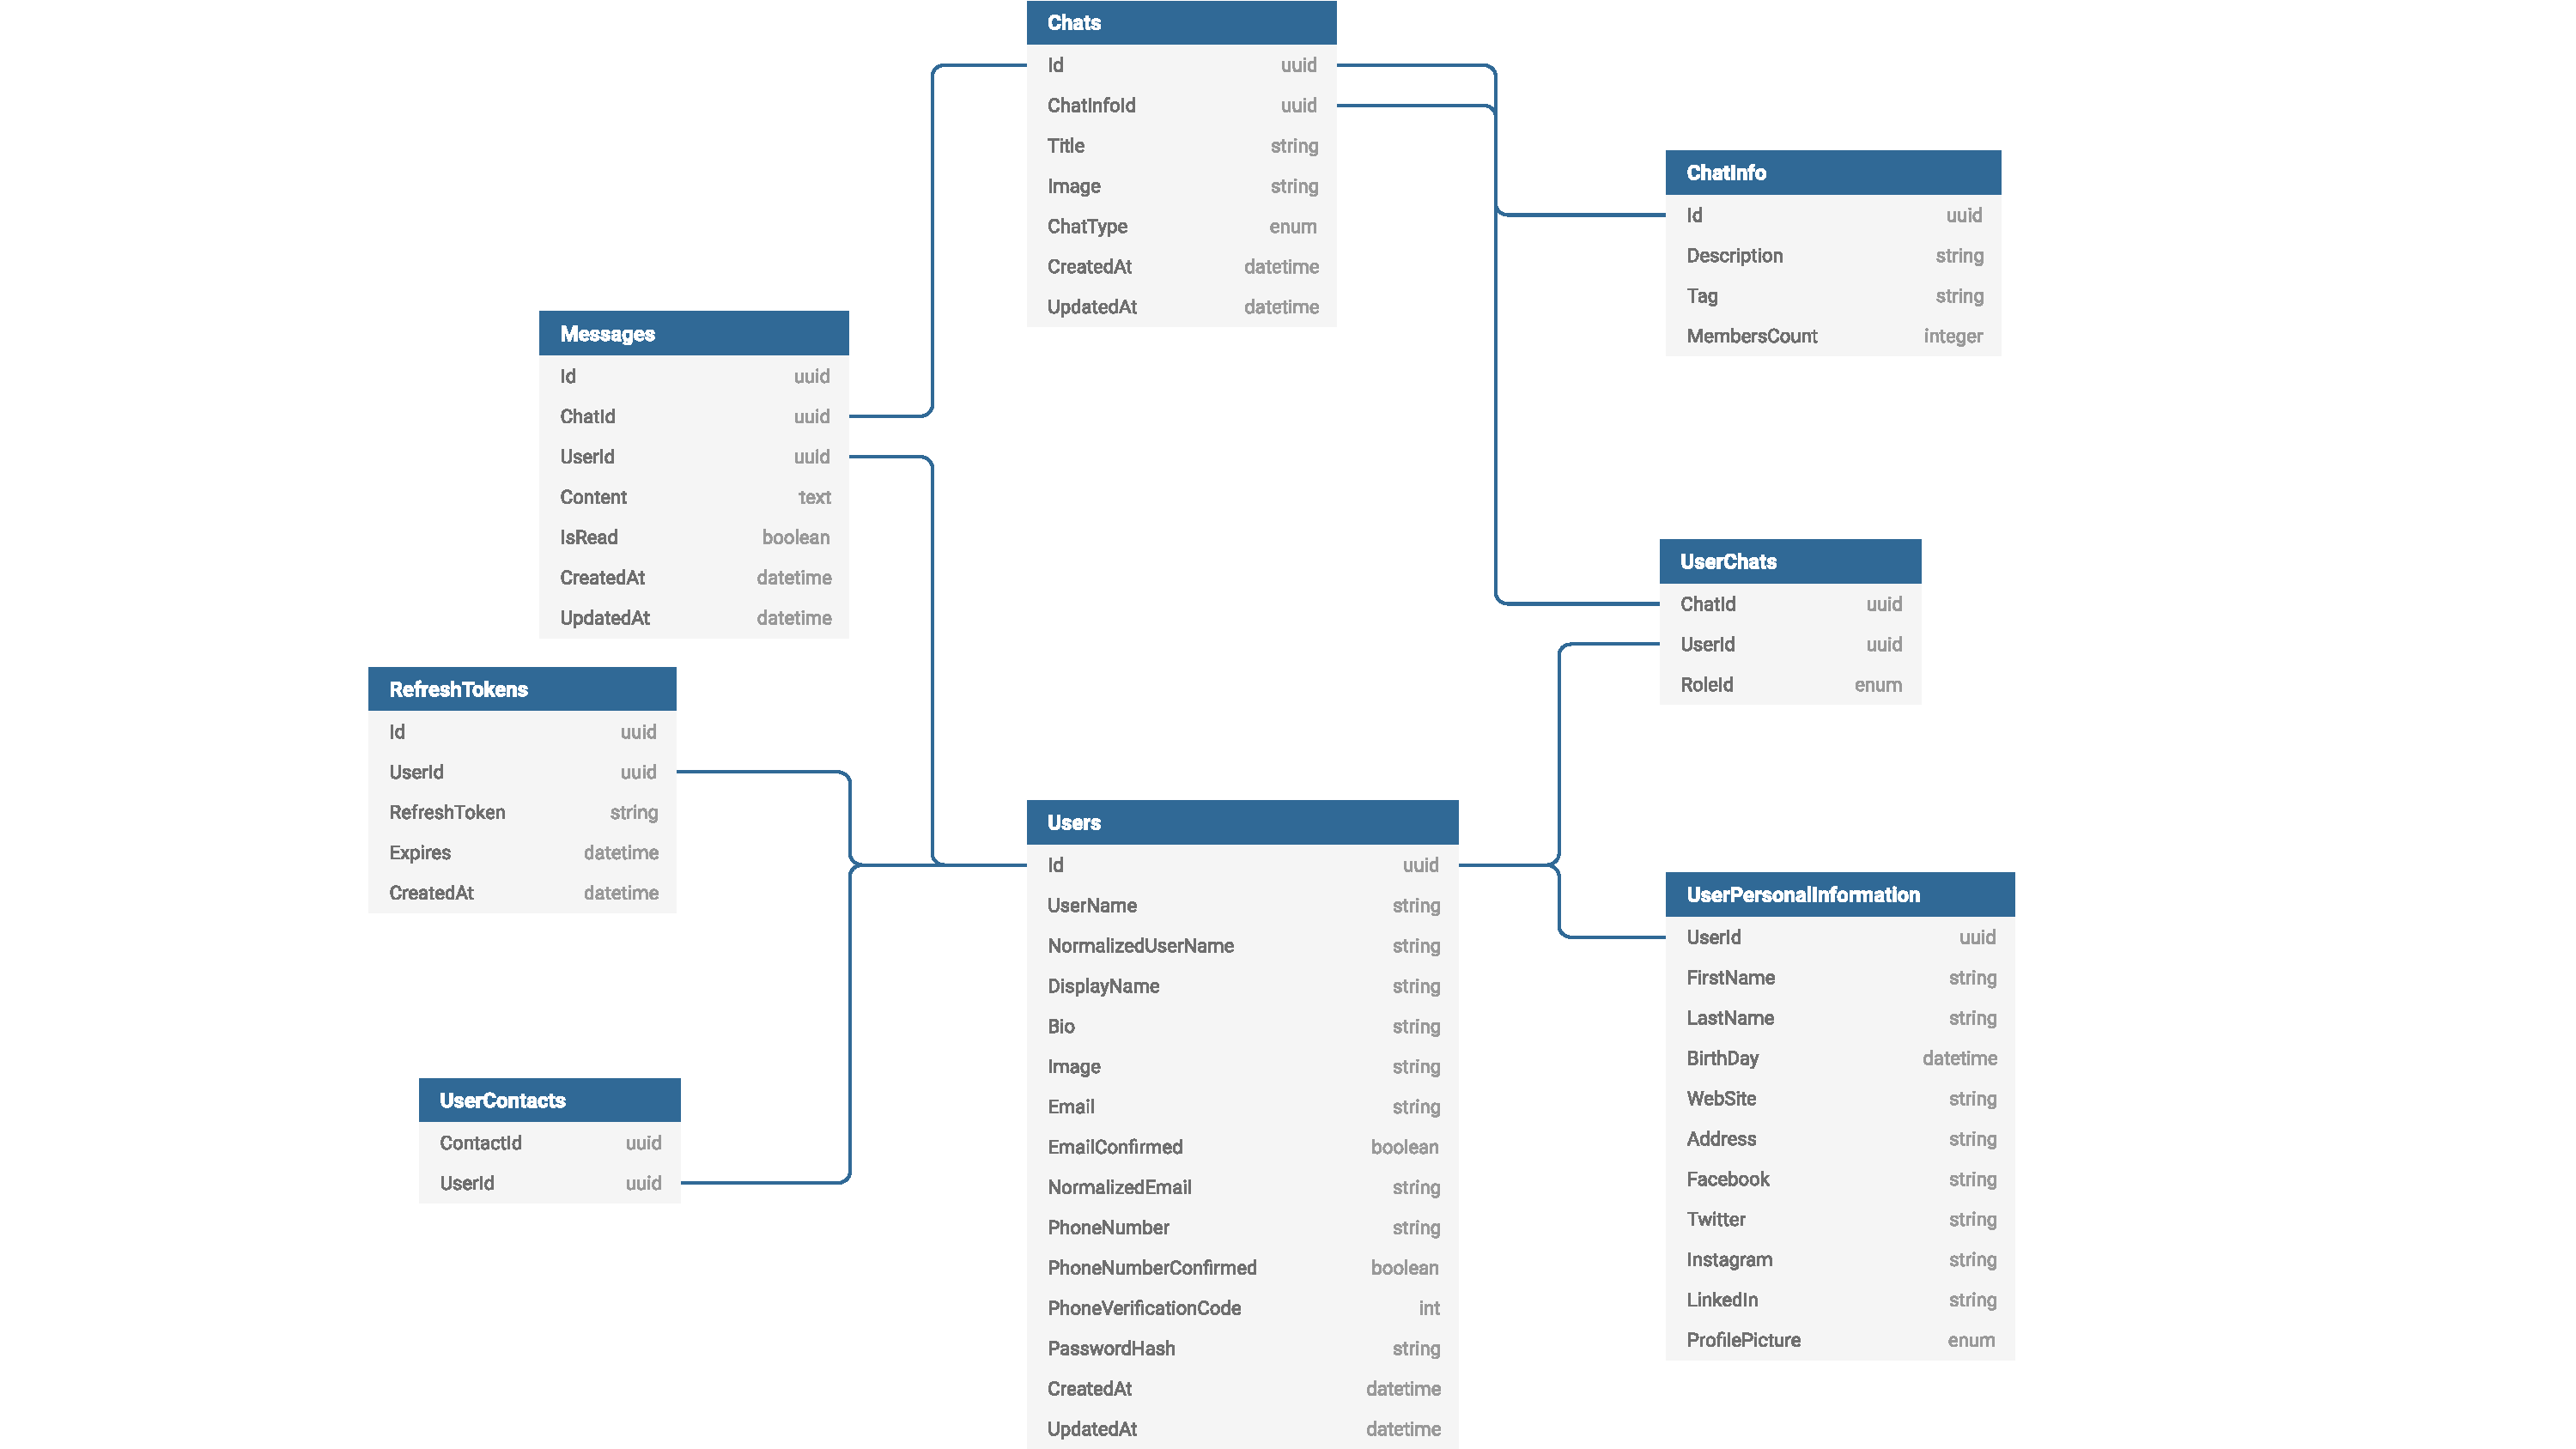
\includegraphics[width=1.2\textwidth]{Pictures/DB_diagram}
    \caption{Database diagram.}\label{fig:figure5}
\end{figure}